\subsection{UC9 - Modifica scaffalatura}
\begin{figure}[H]
  \centering
  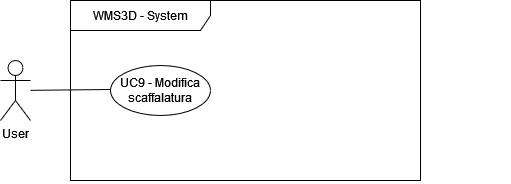
\includegraphics[width=0.8\textwidth]{UC_diagrams_1-10/UC9_sys.drawio.png}
   \caption{Diagramma UML UC9 - Modifica scaffalatura}
\end{figure}
\begin{figure}[H]
  \centering
  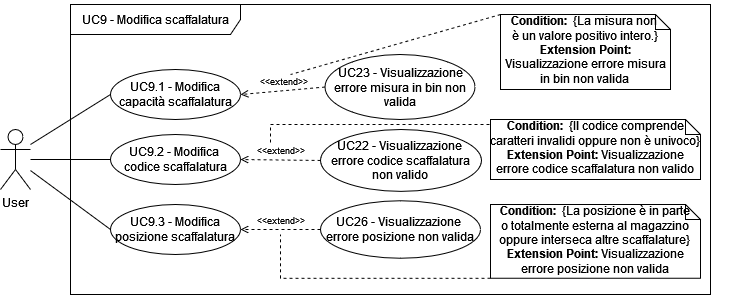
\includegraphics[width=0.8\textwidth]{UC_diagrams_1-10/UC9.drawio.png}
   \caption{Diagramma UML in dettaglio UC9 - Modifica scaffalatura}
\end{figure}
\begin{itemize}
    \item \textbf{Attori:} User.
    \item \textbf{Pre-condizione:}  L'utente ha selezionato una scaffalatura [UC8].
    \item \textbf{Post-condizione:} La scaffalatura viene modificata.
    \item \textbf{Scenario Principale:} L'utente dopo aver selezionato una scaffalatura può modificarne le caratteristiche, in particolare può modificarne la capacità [UC9.1], il codice [UC9.2] oppure la posizione [UC9.3].
    \item \textbf{Generalizzazioni:} -
    \item \textbf{Estensioni:} -
\end{itemize}


\subsubsection{UC9.1 - Modifica capacità scaffalatura}
\begin{figure}[H]
  \centering
  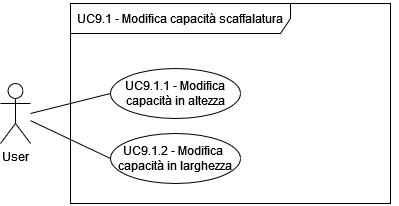
\includegraphics[width=0.8\textwidth]{UC_diagrams_1-10/UC9.1.drawio.png}
   \caption{Diagramma UML UC9.1 - Modifica capacità scaffalatura}
\end{figure}
\begin{itemize}
    \item \textbf{Attori:} User.
    \item \textbf{Pre-condizione:}  L'utente ha selezionato una scaffalatura [UC8] e vuole modificarla.
    \item \textbf{Post-condizione:} Viene modificata la capacità della scaffalatura.
    \item \textbf{Scenario Principale:} L'utente dopo aver selezionato una scaffalatura può modificarne la capacità, in particolare può modificarne la capacità in altezza [UC9.1.1] oppure in larghezza [UC9.1.2].
    \item \textbf{Generalizzazioni:} -
    \item \textbf{Estensioni:} È presente una estensione:
    \begin{itemize}
        \item UC23 - Visualizzazione errore misura in bin non valida.
    \end{itemize}
\end{itemize}


\paragraph{UC9.1.1 - Modifica capacità in altezza}
\begin{figure}[H]
  \centering
  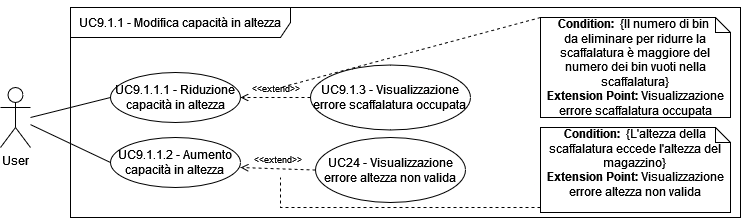
\includegraphics[width=0.8\textwidth]{UC_diagrams_1-10/UC9.1.1.drawio.png}
   \caption{Diagramma UML UC9.1.1 - Modifica capacità in altezza}
\end{figure}
\begin{itemize}
    \item \textbf{Attori:} User.
    \item \textbf{Pre-condizione:} L'utente ha selezionato una scaffalatura [UC8] e vuole modificarne la capacità.
    \item \textbf{Post-condizione:} Viene modificata la capacità in altezza della scaffalatura.
    \item \textbf{Scenario Principale:} L'utente dopo aver selezionato una scaffalatura può modificarne l'altezza, in particolare può decide di ridurre [UC9.1.1.1] o aumentare [UC9.1.1.2] il numero di bin in altezza.
    \item \textbf{Generalizzazioni:} -
    \item \textbf{Estensioni:} -
\end{itemize}


\paragraph{UC9.1.1.1 - Riduzione capacità in altezza}
\begin{itemize}
    \item \textbf{Attori:} User.
    \item \textbf{Pre-condizione:} L'utente ha selezionato una scaffalatura [UC8] e vuole modificarne la capacità in altezza.
    \item \textbf{Post-condizione:} Viene diminuita la capacità in altezza della scaffalatura.
    \item \textbf{Scenario Principale:} L'utente dopo aver selezionato una scaffalatura può ridurre il numero di bin in altezza della scaffalatura.
    \item \textbf{Generalizzazioni:} -
    \item \textbf{Estensioni:} È presente una estensione:
    \begin{itemize}
        \item UC9.1.3 - Visualizzazione errore scaffalatura occupata.
    \end{itemize}
\end{itemize}


\paragraph{UC9.1.1.2 - Aumento capacità in altezza}
\begin{itemize}
    \item \textbf{Attori:} User.
    \item \textbf{Pre-condizione:} L'utente ha selezionato una scaffalatura [UC8] e vuole modificarne la capacità in altezza.
    \item \textbf{Post-condizione:} Viene aumentata la capacità in altezza della scaffalatura.
    \item \textbf{Scenario Principale:} L'utente dopo aver selezionato una scaffalatura può aumentare il numero di bin in altezza della scaffalatura.
    \item \textbf{Generalizzazioni:} -
    \item \textbf{Estensioni:} È presente una estensione:
    \begin{itemize}
        \item UC24 - Visualizzazione errore altezza non valida.
    \end{itemize}
\end{itemize}


\paragraph{UC9.1.2 - Modifica capacità in larghezza}
\begin{figure}[H]
  \centering
  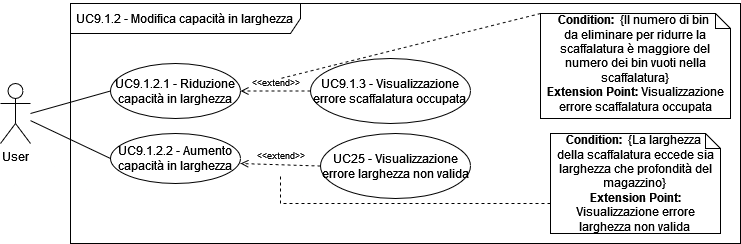
\includegraphics[width=0.8\textwidth]{UC_diagrams_1-10/UC9.1.2.drawio.png}
   \caption{Diagramma UML UC9.1.2 - Modifica capacità in larghezza}
\end{figure}
\begin{itemize}
    \item \textbf{Attori:} User.
    \item \textbf{Pre-condizione:} L'utente ha selezionato una scaffalatura [UC8] e vuole modificarne la capacità.
    \item \textbf{Post-condizione:} Viene modificata la capacità della scaffalatura.
    \item \textbf{Scenario Principale:} L'utente dopo aver selezionato una scaffalatura può modificarne l'altezza, in particolare può decide di ridurre [UC9.1.1.1] o aumentare [UC9.1.1.2] il numero di bin in larghezza.
    \item \textbf{Generalizzazioni:} -
    \item \textbf{Estensioni:} -
\end{itemize}


\paragraph{UC9.1.2.1 - Riduzione capacità in altezza}
\begin{itemize}
    \item \textbf{Attori:} User.
    \item \textbf{Pre-condizione:} L'utente ha selezionato una scaffalatura [UC8] e vuole modificarne la capacità in larghezza.
    \item \textbf{Post-condizione:} Viene diminuita la capacità in larghezza della scaffalatura.
    \item \textbf{Scenario Principale:} L'utente dopo aver selezionato una scaffalatura può ridurre il numero di bin in larghezza della scaffalatura.
    \item \textbf{Generalizzazioni:} -
    \item \textbf{Estensioni:} È presente una estensione:
    \begin{itemize}
        \item UC9.1.3 - Visualizzazione errore scaffalatura occupata.
    \end{itemize}
\end{itemize}


\paragraph{UC9.1.2.2 - Aumento capacità in larghezza}
\begin{itemize}
    \item \textbf{Attori:} User.
    \item \textbf{Pre-condizione:} L'utente ha selezionato una scaffalatura [UC8] e vuole modificarne la capacità in larghezza.
    \item \textbf{Post-condizione:} Viene aumentata la capacità in larghezza della scaffalatura.
    \item \textbf{Scenario Principale:} L'utente dopo aver selezionato una scaffalatura può aumentare il numero di bin in larghezza della scaffalatura.
    \item \textbf{Generalizzazioni:} -
    \item \textbf{Estensioni:} È presente una estensione:
    \begin{itemize}
        \item UC25 - Visualizzazione errore larghezza non valida.
    \end{itemize}
\end{itemize}


\paragraph{UC9.1.3 - Visualizzazione errore scaffalatura occupata}
\begin{itemize}
    \item \textbf{Attori:} User.
    \item \textbf{Pre-condizione:} Si desidera ridurre una scaffalatura, [UC9.1.1.1] o [UC9.1.2.1], per un numero di bin superiore al totale dei bin vuoti.
    \item \textbf{Post-condizione:} L'utente visualizza un messaggio d'errore e l'operazione fallisce.
    \item \textbf{Scenario Principale:} L'utente visualizza un messaggio informativo sull'errore e ne conferma la ricezione. L'operazione fallisce e l'utente dovrà quindi o spostare i prodotti presenti nei bin occupati oppure non ridurre di meno la scaffalatura.
    \item \textbf{Generalizzazioni:} -
    \item \textbf{Estensioni:} -
\end{itemize}


\subsubsection{UC9.2 - Modifica codice scaffalatura}
\begin{itemize}
    \item \textbf{Attori:} User.
    \item \textbf{Pre-condizione:} L'utente ha selezionato una scaffalatura [UC8] e vuole modificarla.
    \item \textbf{Post-condizione:} Viene modificato il codice della scaffalatura.
    \item \textbf{Scenario Principale:} L'utente dopo aver selezionato una scaffalatura può modificarne il codice.
    \item \textbf{Generalizzazioni:} -
    \item \textbf{Estensioni:} È presene una estensione:
    \begin{itemize}
        \item UC22 - Visualizzazione errore codice scaffalatura non valido.
    \end{itemize}
\end{itemize}


\subsubsection{UC9.3 - Modifica posizione scaffalatura}
\begin{itemize}
    \item \textbf{Attori:} User.
    \item \textbf{Pre-condizione:} L'utente ha selezionato una scaffalatura [UC8] e vuole modificarla.
    \item \textbf{Post-condizione:} Viene modificata la posizione della scaffalatura.
    \item \textbf{Scenario Principale:} L'utente dopo aver selezionato una scaffalatura può riposizionare la scaffalatura dove e come vuole all'interno del magazzino.
    \item \textbf{Generalizzazioni:} -
    \item \textbf{Estensioni:} È presente una estensione:
    \begin{itemize}
        \item UC26 - Visualizzazione errore posizione non valida.
    \end{itemize}
\end{itemize}